\documentclass[aspectratio=169, 10pt]{beamer}

\usepackage{bm} % bold math
\usepackage{fontspec}
\usepackage{minted}
\usepackage{pgf-pie}
\usepackage{tikz}

% Custom commands and environments
\makeatletter
\newcommand\version[1]{\renewcommand\@version{#1}}
\newcommand\@version{}
\def\insertversion{\@version}

\newcommand\course[1]{\renewcommand\@course{#1}}
\newcommand\@course{}
\def\insertcourse{\@course}

\newcommand\coursetitle[1]{\renewcommand\@coursetitle{#1}}
\newcommand\@coursetitle{}
\def\insertcoursetitle{\@coursetitle}

\newcommand\lecturenumber[1]{\renewcommand\@lecturenumber{#1}}
\newcommand\@lecturenumber{}
\def\insertlecturenumber{\@lecturenumber}
\makeatother

\newcommand{\slidetitle}[1]{{\xbseries \large \structure{#1}} \bigskip}
\newcommand{\term}[1]{{\color{blue} #1}}
\newcommand{\leftspace}{\hspace{1em}}
\newcommand{\inlinearrow}{
  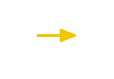
\begin{tikzpicture}[baseline]
    \node [anchor=base] (x) {};
    \draw [rawarrow] (x.mid west) -- ($(x.mid west) + (2em,0)$);
  \end{tikzpicture}
}

\newenvironment{slide}
{\begin{frame}[fragile,environment=slide]\vskip0pt plus 1filll}
{\vskip0pt plus 1filll\end{frame}}

% LaTeX

\setlength{\leftmargini}{1em}

% Common Information

\author{Jon Eyolfson}
\course{ECE 353}
\coursetitle{Systems Software}
\date{2024 Winter}

% fontspec

\defaultfontfeatures{Ligatures=TeX}
% \setmainfont{Domine}
\setsansfont{Inter}[
  FontFace={ul}{n}{Font=*-Thin},
  FontFace={el}{n}{Font=*-ExtraLight},
  FontFace={l}{n}{Font=*-Light},
  FontFace={sb}{n}{Font=*-SemiBold},
  FontFace={eb}{n}{Font=*-ExtraBold},
  FontFace={xb}{n}{Font=*-Black},
]
\setmonofont[Contextuals=AlternateOff, Ligatures=TeXOff]{Iosevka}[
  FontFace={xb}{n}{Font=*-Heavy},
]

%% Font Weights

\DeclareRobustCommand{\ulseries}{\fontseries{ul}\selectfont}
\DeclareTextFontCommand{\textul}{\ulseries}
\DeclareRobustCommand{\elseries}{\fontseries{el}\selectfont}
\DeclareTextFontCommand{\textel}{\elseries}
\DeclareRobustCommand{\lseries}{\fontseries{l}\selectfont}
\DeclareTextFontCommand{\textl}{\lseries}
\DeclareRobustCommand{\sbseries}{\fontseries{sb}\selectfont}
\DeclareTextFontCommand{\textsb}{\sbseries}
\DeclareRobustCommand{\ebseries}{\fontseries{eb}\selectfont}
\DeclareTextFontCommand{\texteb}{\ebseries}
\DeclareRobustCommand{\xbseries}{\fontseries{xb}\selectfont}
\DeclareTextFontCommand{\textxb}{\xbseries}

% tikz

\usetikzlibrary{
  arrows,
  arrows.meta,
  automata,
  backgrounds,
  calc,
  decorations.pathreplacing,
  matrix,
  positioning,
  overlay-beamer-styles,
  shapes,
  shapes.multipart,
  tikzmark,
}

\tikzstyle{rawarrow} = [
  -{Latex[round]},
  line width=1pt,
  yellow,
  shorten >=3pt,
  shorten <=3pt,
  font=\small,
  text=black,
]

\tikzstyle{arrow} = [
  -{Latex[round]},
  line width=1pt,
  yellow,
  shorten >=3pt,
  shorten <=3pt,
  transform canvas={yshift=3pt},
  font=\small,
  text=black,
]

\newcommand{\tikzmarkcoord}[1]{([yshift=3pt]pic cs:#1)}

% minted

\setminted{style=eyolfson, fontsize=\small, escapeinside=||}
\setmintedinline{fontsize=\normalsize}

% hyperref

\hypersetup{colorlinks, urlcolor=blue}

% beamer
\setbeamersize{text margin left=16mm, text margin right=16mm}
\setbeamertemplate{itemize items}[circle]
\setbeamercolor{item}{fg=black}
\setbeamercolor{structure}{fg=darkblue}
\setbeamerfont{frametitle}{series=\bfseries, parent=structure}
\setbeamertemplate{navigation symbols}{}
\setbeamertemplate{headline}{}
\setbeamertemplate{footline}{
  \begin{tikzpicture}[
    remember picture,
    overlay,
    shift={(current page.south west)},
  ]
    \path [fill=gray] (144mm, 0) -- (160mm, 16mm) -- (160mm, 0);
    \node [inner sep=3.5mm, outer sep=0, text=black, anchor=base east,
           align=right, yshift=3.5mm]
          at (current page.south east) {\ttfamily \small \insertframenumber{}};
  \end{tikzpicture}
}
\setbeamertemplate{title page}{
  \begin{tikzpicture}[
    remember picture,
    overlay,
    shift={(current page.south west)},
    background rectangle/.style={fill=darkblue},
    show background rectangle,
  ]
    \node [anchor=center, align=center, text=white, text width=40mm, scale=3.2]
          at (\paperwidth / 2, \paperheight * 2 / 3)
          {\xbseries \inserttitle{}};
    \node [anchor=base west, align=left, inner sep=0, text=white, yshift=2.5mm]
          at (16mm, \paperheight / 3)
          {\insertdate{} \insertcourse{}: \insertcoursetitle{}};
    \node [anchor=base west, align=left, inner sep=0, text=white, yshift=-2.5mm]
          at (16mm, \paperheight / 3)
          {\insertauthor};
    \node [anchor=base east, align=right, inner sep=0, text=white, yshift=2.5mm]
          at (144mm, \paperheight / 3)
          {Lecture \insertlecturenumber{}};
    \node [anchor=base east, align=right, inner sep=0, text=white,
           yshift=-2.5mm]
          at (144mm, \paperheight / 3)
          {\ttfamily \insertversion{}};
    \node [align=center, anchor=south, inner sep=0, text=white, yshift=3.5mm]
          (license) at (\paperwidth / 2, 0)
          {\fontsize{7pt}{7pt}\selectfont This  work is licensed under a
           \href{http://creativecommons.org/licenses/by-sa/4.0/}
                {\color{lightblue} Creative Commons Attribution-ShareAlike 4.0
                 International License}};
  \end{tikzpicture}
}

% xcolor

%% Primary Colour

\definecolor{pantone655}{RGB}{0, 42, 92} % #002a5c
\colorlet{darkblue}{pantone655}

%% Secondary Colours

\definecolor{pantone633}{RGB}{0, 139, 176} % #008bb0
\colorlet{blue}{pantone633}

\definecolor{pantonewarmred}{RGB}{220, 70, 51} % #dc4633
\colorlet{red}{pantonewarmred}

\definecolor{pantone3285}{RGB}{0, 161, 137} % #00a189
\colorlet{cyan}{pantone3285}

\definecolor{pantone7722}{RGB}{13, 83, 77} % #0d534d
\colorlet{darkcyan}{pantone7722}

\definecolor{pantone376}{RGB}{141, 191, 46} % #8dbf2e
\colorlet{green}{pantone376}

\definecolor{pantone2613}{RGB}{109, 36, 122} % #6d247a
\colorlet{violet}{pantone2613}

\definecolor{pantone2985}{RGB}{111, 199, 234} % #6fc7ea
\colorlet{lightblue}{pantone2985}

\definecolor{pantone227}{RGB}{171, 19, 104} % #ab1368
\colorlet{magenta}{pantone227}

\definecolor{pantone7406}{RGB}{241, 197, 0} % #f1c500
\colorlet{yellow}{pantone7406}

%% Neutrals

\definecolor{pantonecoolgray2}{RGB}{208, 209, 201} % #d0d1c9
\colorlet{gray}{pantonecoolgray2}


\lecturenumber{16}
\title{Threads}
\version{2.0.0}

\begin{document}
  \begin{frame}[plain, noframenumbering]
    \titlepage
  \end{frame}

  \begin{slide}

    \slidetitle{Aside: Concurrency and Parallelism Aren't the Same}

    Concurrency

    \leftspace{}Switching between two or more things (can you get interrupted)

    \leftspace{}\leftspace{}Goal: make progress on multiple things
    \medskip

    Parallelism

    \leftspace{}Running two or more things at the same time (are they independent)

    \leftspace{}\leftspace{}Goal: run as fast as possible

  \end{slide}

  \begin{slide}

    \slidetitle{A Real Life Situation of Concurrency and Parallelism}

    You're sitting at a table for dinner, and you can:

    \begin{itemize}
      \item Eat
      \item Drink
      \item Talk
      \item Gesture
    \end{itemize}
    You're so hungry that if you start eating you won't stop until you finish
    \medskip

    Which tasks can and can't be done concurrently, and in parallel?

  \end{slide}

  \begin{slide}

    \slidetitle{Choose Any Two Tasks in the Real Life Example}

    You can't eat and talk (or drink) at the same time, and you can't switch

    \leftspace{}Not parallel and not concurrent
    \medskip

    You could eat and gesture at the same time, but you can't switch

    \leftspace{}Parallel and not concurrent
    \medskip

    You can't drink and talk at the same time, and you could switch

    \leftspace{}Not parallel and concurrent
    \medskip

    You can talk (or drink) and gesture at the same time, and you could switch

    \leftspace{}Parallel and concurrent

  \end{slide}

  \begin{slide}

    \slidetitle{Threads are Like Processes with Shared Memory}

    The same principle as a process, except by default they share memory

    \leftspace{}They have their own registers, program counter, and stack
    \medskip

    They have the same address space, so changes appear in each thread
    \medskip

    You need to explicitly state if any memory is specific to a thread (TLS)

  \end{slide}

  \begin{slide}

    \slidetitle{One Process Can have Multiple Threads}

    By default, a process just executes code in its own address space
    \medskip

    Threads allow multiple executions in the same address space
    \medskip

    They're lighter weight and less expensive to create than processes

    \leftspace{}They share code, data, file descriptors, etc.

  \end{slide}

  \begin{slide}

    \slidetitle{Assuming One CPU, Threads Can Express Concurrency}

    A process can appear like it's executing in multiple locations at once

    \leftspace{}However, the OS is just context switching within a process
    \medskip

    It may be easier to program concurrently

    \leftspace{}e.g., handle a web request in a new thread
    \medskip

    \begin{minted}{c}
while (true) {
  struct request *req = get_request();
  create_thread(process_request, req);
}
    \end{minted}

  \end{slide}

  \begin{slide}

    \slidetitle{Threads are Lighter Weight than Processes}

    \begin{tabular}{ll}
      \textbf{Process} & \textbf{Thread} \\
      \\
      Independent code / data / heap & Shared code / data / heap \\
      \\
      Independent execution & Must live within an executing process \\
      \\
      Has its own stack and registers & Has its own stack and registers \\
      \\
      Expensive creation and context switching & Cheap creation and context switching \\
      \\
      Completely removed from OS on exit & Stack removed from process on exit \\
    \end{tabular}
    \medskip

    When a process dies, all threads within it die as well!

  \end{slide}

  \begin{slide}

    \slidetitle{We'll be Using POSIX Threads}

    For Windows, there's a Win32 thread, but we're going to use *UNIX threads
    \medskip

    \mintinline{c}{#include <pthread.h>} --- in your source file
    \medskip

    \mintinline{c}{-pthread} --- compile and link the pthread library
    \medskip

    All the pthread functions have documentation in the \mintinline{c}{man} pages

  \end{slide}

  \begin{slide}

    \slidetitle{You Create Threads with \texttt{pthread\_create}}

    \begin{minted}{c}
int pthread_create(pthread_t* thread, 
                   const pthread_attr_t* attr,
                   void* (*start_routine)(void*),
                   void* arg);
    \end{minted}
    \medskip

    \begin{tabular}{rl}
      thread & creates a handle to a thread at pointer location \\

      attr & thread attributes (NULL for defaults, more details later) \\

      start\_routine & function to start execution \\

      arg & value to pass to start\_routine \\
    \end{tabular}

    returns 0 on success, error number otherwise
    
    \leftspace{}(contents of *thread are undefined)

  \end{slide}

  \begin{slide}

    \slidetitle{Creating Threads is a Bit Different than Processes}

    \begin{minted}{c}
#include <pthread.h>
#include <stdio.h>

void* run(void*) {
  printf("In run\n");
  return NULL;
}

int main() {
  pthread_t thread;
  pthread_create(&thread, NULL, &run, NULL);
  printf("In main\n");
}
    \end{minted}
    \medskip

    What are some differences? Are we missing anything?

  \end{slide}

  \begin{slide}

    \slidetitle{The \texttt{wait} Equivalent for Threads --- Join}

    \begin{minted}{c}
int pthread_join(pthread_t thread,
                 void** retval)
    \end{minted}
    \medskip

    \begin{tabular}{rp{10cm}}
  thread & wait for this thread to terminate (thread must be joinable) \\

  retval & stores exit status of thread (set by {\tt pthread\_exit}) to
                 the location pointed by *retval. If cancelled returns
                 {\tt PTHREAD\_CANCELED}. {\tt NULL} is ignored. \\
    \end{tabular}

  returns 0 on success, error number otherwise 
  \medskip

  {\bf Only call this one time per thread!}

  \leftspace{}Multiple calls on the same thread leads to undefined behavior

  \end{slide}

  \begin{slide}

    \slidetitle{Previous Example that Waits Properly}

    \begin{minted}{c}
#include <pthread.h>
#include <stdio.h>

void* run(void*) {
  printf("In run\n");
  return NULL;
}

int main() {
  pthread_t thread;
  pthread_create(&thread, NULL, &run, NULL);
  printf("In main\n");
  pthread_join(thread, NULL);
}
    \end{minted}
    \medskip

    Now we joined, the thread's resources are cleaned up

  \end{slide}

  \begin{slide}

    \slidetitle{Ending a Thread Early (Think of \texttt{exit})}

    \begin{minted}{c}
void pthread_exit(void *retval);
    \end{minted}
    \medskip

    \begin{tabular}{rl}
      retval & return value passed to function that calls {\tt pthread\_join} \\
    \end{tabular}
    \medskip
    
    Note: \mintinline{c}{start_routine} returning is equivalent of calling {\tt pthread\_exit}

    \leftspace{}Think of the difference between returning from main and
    \texttt{exit}
    \medskip

    {\tt pthread\_exit} is called implicitly when the {\tt start\_routine} of a
    thread returns

  \end{slide}

  \begin{slide}

    \slidetitle{Detached Threads}

    {\it Joinable} threads (the default) wait for someone to call
    {\tt pthread\_join}

    \leftspace{}then they release their resources
    \medskip

    {\it Detached} threads release their resources when they terminate
    \medskip

    \begin{minted}{c}
int pthread_detach(pthread_t thread);
    \end{minted}
    \medskip

    \begin{tabular}{rl}
      thread & marks the thread as detached \\
    \end{tabular}

    returns 0 on success, error number otherwise
    \medskip

    Calling {\tt pthread\_detach} on an already detached is undefined
    behavior

  \end{slide}

  \begin{slide}

    \slidetitle{Detached Threads Aren't Joined}

    \begin{minted}{c}
#include <pthread.h>
#include <stdio.h>

void* run(void*) {
  printf("In run\n");
  return NULL;
}

int main() {
  pthread_t thread;
  pthread_create(&thread, NULL, &run, NULL);
  pthread_detach(thread);
  printf("In main\n");
}
    \end{minted}
    \medskip

    This code just prints ``In main'', why?

  \end{slide}

  \begin{slide}

    \slidetitle{\texttt{pthread\_exit} in main Waits for All Detached Threads to Finish}

    \begin{minted}{c}
#include <pthread.h>
#include <stdio.h>

void* run(void*) {
  printf("In run\n");
  return NULL;
}

int main() {
  pthread_t thread;
  pthread_create(&thread, NULL, &run, NULL);
  pthread_detach(thread);
  printf("In main\n");
  pthread_exit(NULL);
}
    \end{minted}
    \medskip

    This code now works as expected

  \end{slide}

  \begin{slide}

    \slidetitle{You Can Use Attributes To Get/Set Thread Variables}

    \begin{minted}{c}
size_t stacksize;
pthread_attr_t attributes;
pthread_attr_init(&attributes);
pthread_attr_getstacksize(&attributes, &stacksize);
printf("Stack size = %i\n", stacksize);
pthread_attr_destroy(&attributes);
    \end{minted}

    Running this should show a stack size of 8 MiB (on most Linux systems)
    \medskip

    You can also set a thread state to joinable
    \medskip

    \begin{minted}{c}
pthread_attr_setdetachstate(&attributes,
                            PTHREAD_CREATE_JOINABLE);
    \end{minted}

  \end{slide}

  \begin{slide}

    \slidetitle{Let's Compare Creating Threads to Processes}

    See: \texttt{lectures/16-threads/multiple-thread-example.c}
    \medskip

    Compare this to:
    \texttt{lectures/04-process-creation/multiple-fork-example.c}
    \medskip

    Technically, how should we (very slightly) improve the thread example?

  \end{slide}

  \begin{slide}

    \slidetitle{Threads Enable Concurrency}

    We explored threads, and related them to something we already know (processes)

    \begin{itemize}
      \item Threads are lighter weight, and share memory by default
      \item Each process can have multiple threads (but just one at the start)
    \end{itemize}

  \end{slide}

\end{document}
